\documentclass[9pt,aspectratio=169]{beamer}

% ---------- Packages ----------
\usepackage[utf8]{inputenc}
\usepackage{amsmath,amssymb,amsfonts}
\usepackage{tikz}
\usetikzlibrary{arrows.meta,positioning,calc,decorations.pathreplacing}
\usepackage{mathtools}
\usepackage{booktabs}
\usepackage{array}

% ---------- Theme ----------
\usetheme{Madrid}
\usecolortheme{seahorse}
\setbeamertemplate{navigation symbols}{}
\setbeamertemplate{footline}[frame number]
\setbeamercovered{transparent}

\title[Module 2: Linear Algebra \& Vector Spaces]{Module 2\\ Vectors, Vector Spaces \& Linear Algebra}
\subtitle{Complete Study Notes}
\author{Aishwarya J S}
\institute{M.Tech CSE (AI \& Data Science)}
\date{}

% ---------- Custom commands ----------
\newcommand{\R}{\mathbb{R}}
\newcommand{\vect}[1]{\mathbf{#1}}

\begin{document}

% ================= TITLE =================
\begin{frame}
\titlepage
\end{frame}

% ================= AGENDA =================
\begin{frame}{Module Outline}
\begin{columns}[t]
\column{0.5\textwidth}
\begin{enumerate}
\footnotesize
\item Algebraic Structures
\item Vector Spaces
\item Coordinate Systems \& Vectors
\item Vector Addition \& Scalar Multiplication
\item Linear Combinations, Span, Basis
\item Matrix Multiplication as Composition
\item Three-Dimensional Linear Transformations
\item The Determinant
\item Inverse Matrices, Column Space, Null Space
\end{enumerate}
\column{0.5\textwidth}
\begin{enumerate}
\footnotesize
\setcounter{enumi}{9}
\item Nonsquare Matrices as Transformations
\item Dot Products and Duality
\item Cross Products
\item Cross Products \& Linear Transformations
\item Cramer's Rule
\item Change of Basis
\item Eigenvectors and Eigenvalues
\item Hyperplanes \& Weight Vectors
\item Metric \& Inner Product Spaces
\item Perceptron (Application)
\end{enumerate}
\end{columns}
\end{frame}

% ================================================================
\section{Algebraic Structures}
% ================================================================

\begin{frame}{Set with a Binary Operation}
\begin{block}{Definition}
Let $S$ be a \textbf{set} and $*$ a \textbf{binary operation} on $S$. The pair $(S,*)$ is called an \textbf{algebraic structure}.
\end{block}
\begin{itemize}
\item A binary operation takes two elements of $S$ and combines them to give another element.
\item The properties satisfied by $*$ determine what kind of algebraic structure $(S,*)$ is.
\item This gives a hierarchy: \textbf{Magma $\to$ Semigroup $\to$ Monoid $\to$ Group $\to$ Abelian Group}.
\end{itemize}
\end{frame}

\begin{frame}{Closure Property \& Magma}
\begin{block}{Closure Property}
For all $a, b \in S$: \quad $a * b \in S$.
\end{block}
\begin{alertblock}{Magma}
If $(S,*)$ satisfies the closure property, it is called a \textbf{Magma}.
\end{alertblock}
\begin{itemize}
\item Closure simply means: combining two elements of the set never takes you \emph{outside} the set.
\item Example: $(\mathbb{Z}, +)$ is a magma since the sum of two integers is always an integer.
\end{itemize}
\end{frame}

\begin{frame}{Semigroup}
\begin{block}{Associative Property}
$$a * (b*c) = (a*b) * c \quad \forall\, a,b,c \in S$$
\end{block}
\begin{alertblock}{Semigroup}
A magma $(S,*)$ that also satisfies associativity is called a \textbf{Semigroup}.
\end{alertblock}
\begin{itemize}
\item The order in which we group operations does not matter.
\item Example: $(\mathbb{N}, +)$ is a semigroup.
\end{itemize}
\end{frame}

\begin{frame}{Monoid}
\begin{block}{Identity Element}
There exists $e \in S$ such that
$$a * e = e * a = a \quad \forall\, a \in S$$
\end{block}
\begin{alertblock}{Monoid}
A semigroup with an identity element is called a \textbf{Monoid}.
\end{alertblock}
\begin{itemize}
\item $e$ is called the \textbf{identity element} of the structure.
\item Example: $(\mathbb{Z}, +)$ is a monoid with identity $e = 0$.
\item Example: $(\mathbb{Z}, \times)$ is a monoid with identity $e = 1$.
\end{itemize}
\end{frame}

\begin{frame}{Group}
\begin{block}{Inverse Element}
For every $a \in S$, there exists $a^{-1} \in S$ such that
$$a * a^{-1} = a^{-1} * a = e$$
\end{block}
\begin{alertblock}{Group}
A monoid in which every element has an inverse is called a \textbf{Group}.
\end{alertblock}
\begin{itemize}
\item Every element can be "undone" by combining it with its inverse.
\item Example: $(\mathbb{Z}, +)$ is a group; inverse of $a$ is $-a$.
\item Example: $(\mathbb{Z}, \times)$ is \emph{not} a group (no inverse for most integers).
\end{itemize}
\end{frame}

\begin{frame}{Abelian Group}
\begin{block}{Commutative Property}
$$a * b = b * a \quad \forall\, a,b \in S$$
\end{block}
\begin{alertblock}{Abelian Group}
A group that also satisfies commutativity is called an \textbf{Abelian Group}.
\end{alertblock}
\begin{itemize}
\item Order of combining two elements does not affect the result.
\item Example: $(\mathbb{Z}, +)$ is an abelian group.
\item Example: The set of $n\times n$ invertible matrices under multiplication is a group but \emph{not} abelian (in general).
\end{itemize}
\end{frame}

\begin{frame}{Hierarchy of Algebraic Structures}
\centering
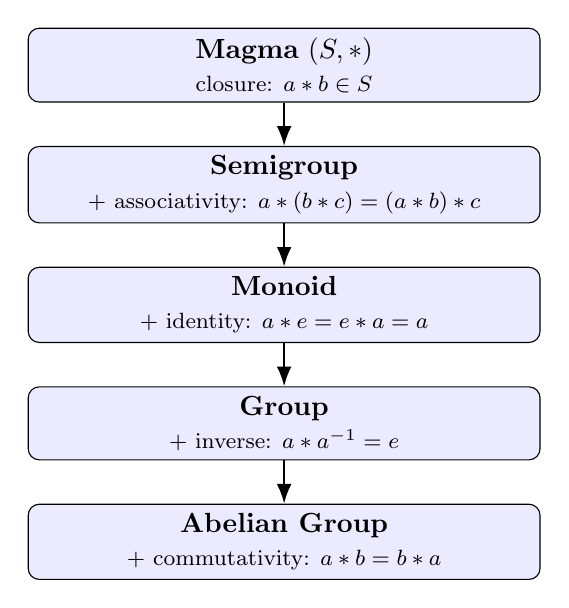
\begin{tikzpicture}[
  node distance=0.55cm and 0.2cm,
  box/.style={draw, rounded corners, minimum width=6.5cm, minimum height=0.9cm, align=center, fill=blue!8},
  lbl/.style={font=\footnotesize\itshape}
]
\node[box] (magma) {\textbf{Magma} $(S,*)$ \\ \footnotesize closure: $a*b \in S$};
\node[box, below=of magma] (semi) {\textbf{Semigroup} \\ \footnotesize $+$ associativity: $a*(b*c)=(a*b)*c$};
\node[box, below=of semi] (mono) {\textbf{Monoid} \\ \footnotesize $+$ identity: $a*e=e*a=a$};
\node[box, below=of mono] (group) {\textbf{Group} \\ \footnotesize $+$ inverse: $a*a^{-1}=e$};
\node[box, below=of group] (abel) {\textbf{Abelian Group} \\ \footnotesize $+$ commutativity: $a*b=b*a$};

\foreach \a/\b in {magma/semi, semi/mono, mono/group, group/abel}
  \draw[-{Latex[length=2.5mm]}, thick] (\a) -- (\b);
\end{tikzpicture}
\end{frame}

\begin{frame}{Ring and Field}
\begin{block}{Ring}
A set with \textbf{two} binary operations (usually $+$ and $\times$) such that:
\begin{itemize}
\item $(S,+)$ is an abelian group,
\item $(S,\times)$ is a semigroup (associative),
\item multiplication distributes over addition.
\end{itemize}
\end{block}
\begin{block}{Field}
A ring in which $(S\setminus\{0\}, \times)$ is also an abelian group (every nonzero element has a multiplicative inverse).
\end{block}
\begin{itemize}
\item Example of a field: $(\mathbb{R}, +, \times)$, $(\mathbb{Q}, +,\times)$, $(\mathbb{C}, +, \times)$.
\item A \textbf{Vector Space} is built from a \textbf{Field} $F$ (scalars) and a set $V$ (vectors) together with vector addition and scalar multiplication: $(V, F, +, \cdot)$.
\end{itemize}
\end{frame}

\begin{frame}{Quick Recap Table: Algebraic Structures}
\centering
\small
\begin{tabular}{@{}lcccc@{}}
\toprule
\textbf{Structure} & Closure & Assoc. & Identity & Inverse \\
\midrule
Magma & \checkmark & & & \\
Semigroup & \checkmark & \checkmark & & \\
Monoid & \checkmark & \checkmark & \checkmark & \\
Group & \checkmark & \checkmark & \checkmark & \checkmark \\
Abelian Group & \checkmark & \checkmark & \checkmark & \checkmark $^{*}$\\
\bottomrule
\end{tabular}
\vspace{0.3cm}
\begin{itemize}
\footnotesize
\item[$^{*}$] Abelian Group additionally requires \textbf{commutativity}: $a*b = b*a$.
\end{itemize}
\end{frame}

% ================================================================
\section{Vector Spaces}
% ================================================================

\begin{frame}{What is a Vector Space?}
\begin{block}{Structure $(V, F, +, \cdot)$}
\begin{itemize}
\item $V$ = set of \textbf{vectors}
\item $F$ = \textbf{scalar field} (e.g. $\mathbb{R}$)
\item $+$ : \textbf{vector addition} \quad ($V \times V \to V$)
\item $\cdot$ : \textbf{scalar multiplication} \quad ($F \times V \to V$)
\end{itemize}
\end{block}
\begin{alertblock}{Definition}
The \textbf{set of all elements} in a vector space is called the set of \textbf{vectors}.
\end{alertblock}
\begin{itemize}
\item Any object that can be described using multiple values can be treated as a vector.
\item Every polynomial is a vector (in the vector space of polynomials).
\end{itemize}
\end{frame}

\begin{frame}{Examples of Vector Spaces}
\begin{itemize}
\item $\R^n$ with usual vector addition and scalar multiplication — the standard example.
\item The set of all $m\times n$ matrices under matrix addition and scalar multiplication.
\item The set of all polynomials of degree $\le n$: e.g. $p(x) = a_0+a_1x+\cdots+a_nx^n$.
\item The set of continuous real-valued functions on $[a,b]$, under pointwise addition and scaling.
\end{itemize}
\begin{alertblock}{Key Insight}
Anything satisfying the 10 vector space axioms — numbers, matrices, polynomials, or functions — can be treated as a "vector," which is what makes linear algebra so widely applicable.
\end{alertblock}
\end{frame}

\begin{frame}{Vector Space Axioms}
For $\vect{u}, \vect{v}, \vect{w} \in V$ and scalars $k, l \in F$:
\begin{columns}[t]
\column{0.5\textwidth}
\footnotesize
\begin{enumerate}
\item $\vect{u}+\vect{v} \in V$ (closure)
\item $\vect{u}+\vect{v} = \vect{v}+\vect{u}$
\item $(\vect{u}+\vect{v})+\vect{w} = \vect{u}+(\vect{v}+\vect{w})$
\item $\exists\, \vect{0}: \vect{u}+\vect{0}=\vect{u}$
\item $\exists\, -\vect{u}: \vect{u}+(-\vect{u}) = \vect{0}$
\end{enumerate}
\column{0.5\textwidth}
\footnotesize
\begin{enumerate}
\setcounter{enumi}{5}
\item $k\vect{u} \in V$ (closure under scalar mult.)
\item $k(\vect{u}+\vect{v}) = k\vect{u}+k\vect{v}$
\item $(k+l)\vect{u} = k\vect{u}+l\vect{u}$
\item $k(l\vect{u}) = (kl)\vect{u}$
\item $1\cdot \vect{u} = \vect{u}$
\end{enumerate}
\end{columns}
\vspace{0.3cm}
\begin{itemize}
\item Any object that can be "vectorised" with $n$-valued vectors and satisfies these axioms forms a vector space.
\end{itemize}
\end{frame}

\begin{frame}{Vectors: Direction and Magnitude}
\begin{alertblock}{Key Idea}
Any object described using \textbf{multiple values} — a \textbf{Vector} — will always have a \textbf{direction} and a \textbf{magnitude}.
\end{alertblock}
\begin{exampleblock}{Example}
$$V = \begin{bmatrix} 2 \\ 3 \end{bmatrix}, \qquad k = 3$$
$$k \cdot V = 3\begin{bmatrix} 2 \\ 3 \end{bmatrix} = \begin{bmatrix} 6 \\ 9 \end{bmatrix}$$
\end{exampleblock}
\begin{itemize}
\item \textbf{Scalar multiplication changes the magnitude of a vector} (and, if $k<0$, reverses its direction).
\end{itemize}
\end{frame}

% ================================================================
\section{Coordinate Systems \& Vectors}
% ================================================================

\begin{frame}{Coordinate System and Vectors}
\begin{itemize}
\item A \textbf{coordinate system} lets us represent a vector as an ordered tuple of numbers (its components) relative to chosen basis directions.
\item In $\R^2$: $\vect{v} = (x,y)$; in $\R^n$: $\vect{v} = (x_1, x_2, \dots, x_n)$.
\item Each vector can be visualised as an arrow from the origin to the point given by its coordinates.
\end{itemize}
\centering
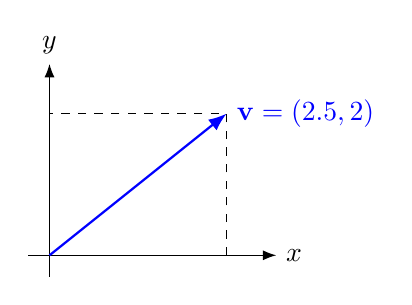
\begin{tikzpicture}[scale=0.9]
\draw[-{Latex}] (-0.3,0) -- (3.2,0) node[right]{$x$};
\draw[-{Latex}] (0,-0.3) -- (0,2.7) node[above]{$y$};
\draw[-{Latex}, thick, blue] (0,0) -- (2.5,2) node[right]{$\vect{v}=(2.5,2)$};
\draw[dashed] (2.5,0) -- (2.5,2) -- (0,2);
\end{tikzpicture}
\end{frame}

\begin{frame}{Vector Addition (Parallelogram / Triangle Law)}
\begin{block}{Rule}
The \textbf{resultant vector} of two vectors becomes the \textbf{diagonal of the parallelogram} formed by the two vectors.
\end{block}
\begin{exampleblock}{Example}
$$\vect{r}_1=(3,5,2), \quad \vect{r}_2=(1,3,4)$$
$$\vect{r}_1+\vect{r}_2 = (4,8,6)$$
\end{exampleblock}
\centering
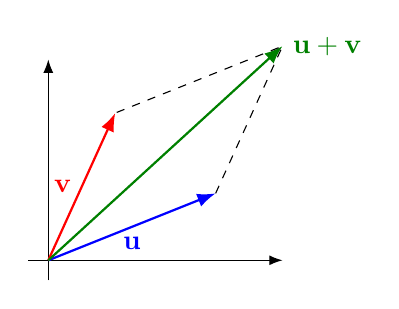
\begin{tikzpicture}[scale=0.85]
\draw[-{Latex}] (-0.3,0) -- (3.5,0);
\draw[-{Latex}] (0,-0.3) -- (0,3);
\draw[-{Latex}, thick, blue] (0,0) -- (2.5,1) node[midway, below]{$\vect{u}$};
\draw[-{Latex}, thick, red] (0,0) -- (1,2.2) node[midway, left]{$\vect{v}$};
\draw[-{Latex}, thick, green!50!black] (0,0) -- (3.5,3.2) node[right]{$\vect{u}+\vect{v}$};
\draw[dashed] (2.5,1) -- (3.5,3.2) -- (1,2.2);
\end{tikzpicture}
\end{frame}

\begin{frame}{Vector Subtraction \& Distance}
\begin{block}{Definition}
$$\vect{PQ} = \vect{Q}-\vect{P} = \vect{v}-\vect{u}$$
If $\vect{u}=(u_1,u_2)$, $\vect{v}=(v_1,v_2)$: \quad $\vect{PQ} = (v_1-u_1,\, v_2-u_2)$
\end{block}
\begin{block}{Squared Norm of $\vect{PQ}$}
\begin{align*}
\|\vect{PQ}\|^2 &= (v_1-u_1)^2+(v_2-u_2)^2\\
&= (v_1^2+v_2^2)+(u_1^2+u_2^2) - 2(v_1u_1+v_2u_2)\\
&= \|\vect{v}\|^2+\|\vect{u}\|^2 - 2\langle \vect{u},\vect{v}\rangle
\end{align*}
\end{block}
This is exactly the \textbf{Law of Cosines}: $\;v^2+u^2-2uv\cos\theta$.
\end{frame}

% ================================================================
\section{Linear Combinations, Span \& Basis}
% ================================================================

\begin{frame}{Linear Combination}
\begin{block}{Definition}
A \textbf{linear combination} of vectors $\vect{v}_1, \vect{v}_2, \dots, \vect{v}_n$ is any vector of the form
$$c_1\vect{v}_1 + c_2\vect{v}_2 + \cdots + c_n\vect{v}_n$$
where $c_1, \dots, c_n$ are scalars.
\end{block}
\begin{itemize}
\item Scaling and adding vectors together produces new vectors.
\item Every vector in $\R^2$ can be written as a linear combination of $\hat{i}=(1,0)$ and $\hat{j}=(0,1)$.
\end{itemize}
\end{frame}

\begin{frame}{Span}
\begin{block}{Definition}
The \textbf{span} of a set of vectors is the set of \textbf{all possible linear combinations} of those vectors.
$$\text{span}(\vect{v}_1,\dots,\vect{v}_n) = \{c_1\vect{v}_1+\cdots+c_n\vect{v}_n : c_i \in F\}$$
\end{block}
\begin{itemize}
\item Span of one nonzero vector in $\R^2$ $\to$ a line through the origin.
\item Span of two non-parallel vectors in $\R^2$ $\to$ the entire plane $\R^2$.
\item If a vector's direction can be produced by scaling and adding others, it lies in their span.
\end{itemize}
\end{frame}

\begin{frame}{Basis}
\begin{block}{Definition}
A \textbf{basis} of a vector space $V$ is a set of \textbf{linearly independent} vectors that \textbf{span} $V$.
\end{block}
\begin{itemize}
\item \textbf{Linear independence}: no vector in the set can be written as a linear combination of the others.
\item Every vector in $V$ can be written \textbf{uniquely} as a linear combination of basis vectors.
\item \textbf{Standard basis} of $\R^n$: $\{e_1, e_2, \dots, e_n\}$ where $e_i$ has $1$ in position $i$ and $0$ elsewhere.
\item The number of vectors in a basis = \textbf{dimension} of the vector space.
\end{itemize}
\end{frame}

\begin{frame}{Worked Example: Linear Combination}
\begin{exampleblock}{Problem}
Express $\vect{v}=(7,4)$ as a linear combination of $\vect{v}_1=(2,1)$ and $\vect{v}_2=(1,2)$.
\end{exampleblock}
\begin{block}{Solution}
Solve $c_1(2,1)+c_2(1,2) = (7,4)$:
$$2c_1+c_2 = 7, \qquad c_1+2c_2 = 4$$
Solving: $c_1 = 10/3,\; c_2 = 1/3$ (approx.), or use exact elimination to get the required scalars.
\end{block}
\begin{itemize}
\item Since $\vect{v}_1,\vect{v}_2$ are linearly independent and span $\R^2$, \emph{every} vector in $\R^2$ can be written this way — confirming $\{\vect{v}_1,\vect{v}_2\}$ is a basis.
\end{itemize}
\end{frame}

\begin{frame}{Example: Span and Basis in $\R^2$}
\begin{exampleblock}{Standard Basis}
$$e_1 = \begin{bmatrix}1\\0\end{bmatrix}, \quad e_2 = \begin{bmatrix}0\\1\end{bmatrix}$$
Any $\vect{v}=(x,y) = x\,e_1 + y\,e_2$.
\end{exampleblock}
\begin{exampleblock}{Another Basis}
$$\vect{b}_1=\begin{bmatrix}1\\1\end{bmatrix}, \quad \vect{b}_2 = \begin{bmatrix}1\\-1\end{bmatrix}$$
These are linearly independent and span $\R^2$, so they also form a valid basis.
\end{exampleblock}
\end{frame}

% ================================================================
\section{Matrix Multiplication as Composition}
% ================================================================

\begin{frame}{Matrices as Linear Transformations}
\begin{itemize}
\item A matrix $A$ represents a \textbf{linear transformation} $T:\R^n \to \R^m$, where $T(\vect{x}) = A\vect{x}$.
\item Columns of $A$ tell us where the basis vectors land after the transformation.
\end{itemize}
\begin{block}{Matrix Multiplication = Composition of Transformations}
If $A$ represents transformation $T_1$ and $B$ represents $T_2$, then the product $AB$ represents applying $T_2$ \textbf{first}, then $T_1$:
$$(AB)\vect{x} = A(B\vect{x}) = T_1(T_2(\vect{x}))$$
\end{block}
\begin{itemize}
\item Order matters: $AB \neq BA$ in general, since composing transformations in a different order gives a different result.
\end{itemize}
\end{frame}

\begin{frame}{Example: Composition of Transformations}
\begin{exampleblock}{Rotation then Shear}
$$A = \begin{bmatrix}1 & 1\\ 0 & 1\end{bmatrix} \text{(shear)}, \qquad B = \begin{bmatrix}0 & -1\\ 1 & 0\end{bmatrix}\text{(90$^\circ$ rotation)}$$
$$AB = \begin{bmatrix}1 & 1\\ 0 & 1\end{bmatrix}\begin{bmatrix}0 & -1\\ 1 & 0\end{bmatrix} = \begin{bmatrix}1 & -1\\ 1 & 0\end{bmatrix}$$
\end{exampleblock}
\begin{itemize}
\item Applying $AB$ to $\vect{x}$ is the same as first rotating $\vect{x}$ by $B$, then shearing the result by $A$.
\end{itemize}
\end{frame}

\begin{frame}{Visualising a Linear Transformation}
\centering
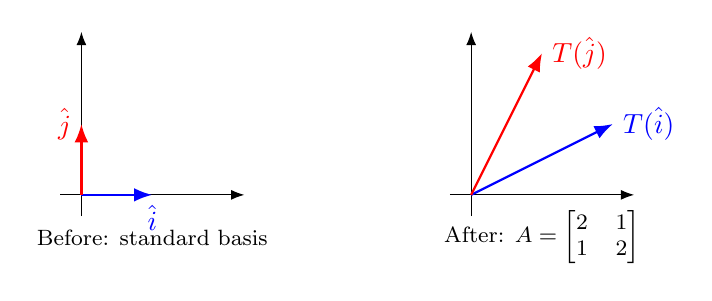
\begin{tikzpicture}[scale=0.9]
\begin{scope}
\draw[-{Latex}] (-0.3,0) -- (2.3,0);
\draw[-{Latex}] (0,-0.3) -- (0,2.3);
\draw[-{Latex}, thick, blue] (0,0) -- (1,0) node[below]{$\hat i$};
\draw[-{Latex}, thick, red] (0,0) -- (0,1) node[left]{$\hat j$};
\node at (1,-0.6) {\footnotesize Before: standard basis};
\end{scope}
\begin{scope}[xshift=5.5cm]
\draw[-{Latex}] (-0.3,0) -- (2.3,0);
\draw[-{Latex}] (0,-0.3) -- (0,2.3);
\draw[-{Latex}, thick, blue] (0,0) -- (2,1) node[right]{$T(\hat i)$};
\draw[-{Latex}, thick, red] (0,0) -- (1,2) node[right]{$T(\hat j)$};
\node at (1,-0.6) {\footnotesize After: $A=\begin{bmatrix}2&1\\1&2\end{bmatrix}$};
\end{scope}
\end{tikzpicture}
\begin{itemize}
\item The columns of the transformation matrix show exactly where each basis vector lands.
\item Every other vector transforms accordingly, since $T$ is linear: $T(\vect{x}) = A\vect{x}$.
\end{itemize}
\end{frame}

% ================================================================
\section{Three-Dimensional Linear Transformations}
% ================================================================

\begin{frame}{Three-Dimensional Linear Transformations}
\begin{itemize}
\item A linear transformation $T:\R^3\to\R^3$ is represented by a $3\times 3$ matrix.
\item Each column shows where $\hat{i}, \hat{j}, \hat{k}$ (standard basis vectors) land.
\end{itemize}
\begin{block}{General Form}
$$T\begin{bmatrix}x\\y\\z\end{bmatrix} = \begin{bmatrix}a&b&c\\d&e&f\\g&h&i\end{bmatrix}\begin{bmatrix}x\\y\\z\end{bmatrix}$$
where columns $(a,d,g)$, $(b,e,h)$, $(c,f,i)$ are the images of $\hat i, \hat j, \hat k$.
\end{block}
\begin{itemize}
\item Composition of 3D transformations again corresponds to matrix multiplication.
\item The determinant of the $3\times3$ matrix gives the \textbf{volume scaling factor} of the transformation.
\end{itemize}
\end{frame}

% ================================================================
\section{The Determinant}
% ================================================================

\begin{frame}{The Determinant}
\begin{block}{Meaning}
The \textbf{determinant} of a matrix measures how much a linear transformation \textbf{scales area (2D)} or \textbf{volume (3D)}.
\end{block}
\begin{itemize}
\item $\det(A) = 0 \iff$ the transformation squashes space into a lower dimension (columns are linearly dependent).
\item Negative determinant $\Rightarrow$ orientation of space is flipped.
\end{itemize}
\begin{exampleblock}{$2\times 2$ Determinant}
$$A=\begin{bmatrix}a&b\\c&d\end{bmatrix}, \qquad \det(A) = ad-bc$$
\end{exampleblock}
\begin{exampleblock}{$3\times 3$ Determinant (cofactor expansion)}
$$\det(A) = a(ei-fh) - b(di-fg) + c(dh-eg)$$
\end{exampleblock}
\end{frame}

\begin{frame}{Properties of the Determinant}
\begin{itemize}
\item $\det(AB) = \det(A)\det(B)$
\item $\det(A^{-1}) = \dfrac{1}{\det(A)}$ \quad (only exists if $\det(A)\neq 0$)
\item $\det(A^T) = \det(A)$
\item Swapping two rows/columns flips the sign of the determinant.
\item A matrix is \textbf{invertible} $\iff$ $\det(A)\neq 0$.
\end{itemize}
\end{frame}

% ================================================================
\section{Inverse Matrices, Column Space, Null Space}
% ================================================================

\begin{frame}{Inverse Matrices}
\begin{block}{Definition}
$A^{-1}$ is the matrix such that
$$A A^{-1} = A^{-1}A = I$$
\end{block}
\begin{itemize}
\item Applying $A^{-1}$ \textbf{undoes} the transformation done by $A$.
\item $A^{-1}$ exists only when $\det(A) \neq 0$ (i.e. $A$ is \textbf{nonsingular}).
\item Used to solve linear systems: $A\vect{x}=\vect{b} \Rightarrow \vect{x} = A^{-1}\vect{b}$.
\end{itemize}
\begin{exampleblock}{$2\times 2$ Inverse Formula}
$$A=\begin{bmatrix}a&b\\c&d\end{bmatrix}, \qquad A^{-1} = \frac{1}{ad-bc}\begin{bmatrix}d&-b\\-c&a\end{bmatrix}$$
\end{exampleblock}
\end{frame}

\begin{frame}{Column Space}
\begin{block}{Definition}
The \textbf{column space} of $A$, $\text{Col}(A)$, is the \textbf{span of the columns} of $A$ — i.e., the set of all possible outputs $A\vect{x}$.
\end{block}
\begin{itemize}
\item Tells us the set of vectors "reachable" by the transformation.
\item $\dim(\text{Col}(A)) = \text{rank}(A)$.
\item If $\text{rank}(A) = n$ (full column rank), the transformation is \textbf{injective} (one-to-one).
\end{itemize}
\end{frame}

\begin{frame}{Null Space}
\begin{block}{Definition}
The \textbf{null space} of $A$, $\text{Null}(A)$, is the set of all vectors that map to the \textbf{zero vector}:
$$\text{Null}(A) = \{\vect{x} : A\vect{x} = \vect{0}\}$$
\end{block}
\begin{itemize}
\item Represents the vectors that get "squashed" to the origin.
\item If $\text{Null}(A) = \{\vect{0}\}$ only, the transformation is injective.
\end{itemize}
\begin{block}{Rank–Nullity Theorem}
$$\text{rank}(A) + \text{nullity}(A) = n \quad (\text{number of columns of } A)$$
\end{block}
\end{frame}

\begin{frame}{Worked Example: Column Space \& Null Space}
\begin{exampleblock}{Problem}
$$A = \begin{bmatrix}1&2\\2&4\end{bmatrix}$$
\end{exampleblock}
\begin{block}{Solution}
\begin{itemize}
\item Columns $(1,2)$ and $(2,4)$ are parallel $\Rightarrow$ $\text{rank}(A)=1$.
\item $\text{Col}(A) = \text{span}\{(1,2)\}$ — a line through the origin.
\item $\text{Null}(A)$: solve $A\vect{x}=0 \Rightarrow x_1 = -2x_2 \Rightarrow \text{Null}(A) = \text{span}\{(-2,1)\}$.
\item Check rank–nullity: $\text{rank}(A) + \text{nullity}(A) = 1+1 = 2 = n$. \checkmark
\end{itemize}
\end{block}
\end{frame}

% ================================================================
\section{Nonsquare Matrices as Transformations}
% ================================================================

\begin{frame}{Nonsquare Matrices: Transformations Between Dimensions}
\begin{itemize}
\item An $m \times n$ matrix represents a transformation $T: \R^n \to \R^m$.
\item If $m > n$: maps a \textbf{lower-dimensional} space into a \textbf{higher-dimensional} one (e.g. $\R^2 \to \R^3$ embeds a plane in 3D space).
\item If $m < n$: maps a \textbf{higher-dimensional} space into a \textbf{lower-dimensional} one (e.g. $\R^3 \to \R^2$ projects 3D onto a plane).
\end{itemize}
\begin{exampleblock}{Example: $\R^2 \to \R^3$}
$$A = \begin{bmatrix}1&0\\0&1\\1&1\end{bmatrix}, \qquad A\begin{bmatrix}x\\y\end{bmatrix} = \begin{bmatrix}x\\y\\x+y\end{bmatrix}$$
\end{exampleblock}
The determinant is not defined for nonsquare matrices; instead we talk about \textbf{rank}.
\end{frame}

% ================================================================
\section{Dot Products and Duality}
% ================================================================

\begin{frame}{Dot Product}
\begin{block}{Definition}
$$\vect{u}\cdot \vect{v} = u_1v_1+u_2v_2+\cdots+u_nv_n = \|\vect{u}\|\,\|\vect{v}\|\cos\theta$$
\end{block}
\begin{itemize}
\item Measures how much two vectors point in the \textbf{same direction}.
\item $\vect{u}\cdot\vect{v} = 0 \iff \vect{u} \perp \vect{v}$ (\textbf{orthogonal}).
\item $\vect{u}\cdot\vect{v} > 0$: vectors point in similar direction; $<0$: opposite direction.
\end{itemize}
\begin{alertblock}{Perpendicular Line/Plane Rule}
For line $ax+by+c=0$: normal vector is $(a,b)$. \\
For plane $ax+by+cz+d=0$: normal vector is $(a,b,c)$.
\end{alertblock}
\end{frame}

\begin{frame}{Dot Product: Projection Formula}
\begin{block}{Scalar Projection of $\vect{u}$ onto $\vect{v}$}
$$\text{comp}_{\vect{v}}\vect{u} = \frac{\vect{u}\cdot\vect{v}}{\|\vect{v}\|}$$
\end{block}
\begin{block}{Vector Projection}
$$\text{proj}_{\vect{v}}\vect{u} = \frac{\vect{u}\cdot\vect{v}}{\|\vect{v}\|^2}\,\vect{v}$$
\end{block}
\begin{itemize}
\item Gives the "shadow" of $\vect{u}$ falling along the direction of $\vect{v}$.
\item Used to decompose a vector into components parallel and perpendicular to another vector.
\end{itemize}
\end{frame}

\begin{frame}{Duality: Dot Products as Linear Transformations}
\begin{block}{Duality Principle}
Every linear transformation from $\R^n \to \R$ (a $1\times n$ matrix) corresponds to a unique vector $\vect{w}$ such that the transformation is the dot product with $\vect{w}$:
$$T(\vect{x}) = \vect{w}\cdot \vect{x} = \vect{w}^T \vect{x}$$
\end{block}
\begin{itemize}
\item This is why $1\times n$ matrices (row vectors) and $n$-dimensional vectors are "dual" to each other.
\item Every dot product can be viewed as first applying the linear transformation $\vect{w}^T$, then reading off the single number result.
\end{itemize}
\end{frame}

\begin{frame}{Perpendicularity via Dot Product}
\centering
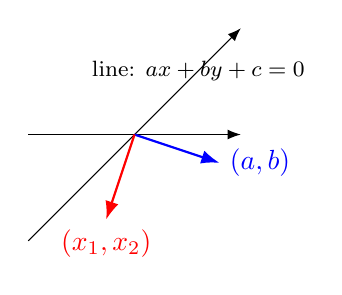
\begin{tikzpicture}[scale=0.9]
\draw[-{Latex}] (-1.5,0) -- (1.5,0);
\draw[-{Latex}] (-1.5,-1.5) -- (1.5,1.5);
\draw[-{Latex}, thick, blue] (0,0) -- (1.2,-0.4) node[right]{$(a,b)$};
\draw[-{Latex}, thick, red] (0,0) -- (-0.4,-1.2) node[below]{$(x_1,x_2)$};
\node at (0.9,0.9) {\footnotesize line: $ax+by+c=0$};
\end{tikzpicture}
\begin{block}{Key Relations}
\begin{itemize}
\item Line: $ax+by+c=0 \;\Rightarrow\; \vect{w}=(a,b) \perp$ the line's direction vector.
\item Hyperplane in $\R^n$: $\displaystyle\sum_{i=1}^n w_ix_i + \theta = 0 \;\Leftrightarrow\; \vect{w}^T\vect{x}+\theta = 0$
\end{itemize}
\end{block}
\end{frame}

% ================================================================
\section{Cross Products}
% ================================================================

\begin{frame}{Cross Product}
\begin{block}{Definition (in $\R^3$)}
$$\vect{u}\times \vect{v} = \begin{vmatrix} \hat{i} & \hat{j} & \hat{k} \\ u_1&u_2&u_3\\ v_1&v_2&v_3\end{vmatrix}$$
\end{block}
\begin{itemize}
\item Produces a vector \textbf{perpendicular to both} $\vect{u}$ and $\vect{v}$ (right-hand rule gives direction).
\item Magnitude: $\|\vect{u}\times\vect{v}\| = \|\vect{u}\|\|\vect{v}\|\sin\theta$ = \textbf{area of the parallelogram} spanned by $\vect{u}, \vect{v}$.
\item $\vect{u}\times\vect{v} = \vect{0} \iff \vect{u}, \vect{v}$ are parallel.
\item \textbf{Anti-commutative}: $\vect{u}\times\vect{v} = -(\vect{v}\times\vect{u})$.
\end{itemize}
\end{frame}

\begin{frame}{Cross Products in Light of Linear Transformations}
\begin{itemize}
\item The cross product with a fixed vector $\vect{u}$, i.e. $T(\vect{v}) = \vect{u}\times\vect{v}$, is itself a \textbf{linear transformation} $\R^3\to\R^3$.
\item This transformation can be represented by a matrix (via the "duality"/determinant trick):
$$\vect{u}\times\vect{v} = \begin{bmatrix}0&-u_3&u_2\\u_3&0&-u_1\\-u_2&u_1&0\end{bmatrix}\begin{bmatrix}v_1\\v_2\\v_3\end{bmatrix}$$
\item The \textbf{scalar triple product} $\vect{a}\cdot(\vect{b}\times\vect{c})$ equals the determinant of the matrix with rows $\vect{a},\vect{b},\vect{c}$, and gives the \textbf{volume} of the parallelepiped they span.
\end{itemize}
\end{frame}

\begin{frame}{Worked Example: Cross Product}
\begin{exampleblock}{Problem}
$$\vect{u}=(1,0,0), \qquad \vect{v}=(0,1,0)$$
\end{exampleblock}
\begin{block}{Solution}
$$\vect{u}\times\vect{v} = \begin{vmatrix}\hat i&\hat j&\hat k\\1&0&0\\0&1&0\end{vmatrix} = \hat k = (0,0,1)$$
\end{block}
\begin{itemize}
\item Magnitude $= \|\vect{u}\|\|\vect{v}\|\sin(90^\circ) = 1$ = area of the unit square spanned by $\hat i,\hat j$.
\item Direction $(0,0,1)$ is perpendicular to both $\vect{u}$ and $\vect{v}$, confirmed by the right-hand rule.
\end{itemize}
\end{frame}

% ================================================================
\section{Cramer's Rule}
% ================================================================

\begin{frame}{Cramer's Rule}
\begin{block}{Statement}
For the system $A\vect{x}=\vect{b}$ with $\det(A)\neq 0$, each variable $x_i$ is given by
$$x_i = \frac{\det(A_i)}{\det(A)}$$
where $A_i$ is $A$ with column $i$ replaced by $\vect{b}$.
\end{block}
\begin{exampleblock}{Example}
$$\begin{cases} 2x+y=5\\ x-y=1\end{cases} \Rightarrow A=\begin{bmatrix}2&1\\1&-1\end{bmatrix},\; \det(A)=-3$$
$$x = \frac{\begin{vmatrix}5&1\\1&-1\end{vmatrix}}{-3} = \frac{-6}{-3}=2, \qquad y = \frac{\begin{vmatrix}2&5\\1&1\end{vmatrix}}{-3} = \frac{-3}{-3}=1$$
\end{exampleblock}
\end{frame}

% ================================================================
\section{Change of Basis}
% ================================================================

\begin{frame}{Change of Basis}
\begin{itemize}
\item A vector's \textbf{coordinates} depend on the chosen basis; the vector itself doesn't change.
\item If $B = \{\vect{b}_1, \vect{b}_2, \dots\}$ is a new basis, then the \textbf{change-of-basis matrix} has $\vect{b}_i$ as its columns.
\end{itemize}
\begin{block}{Translating Coordinates}
If $[\vect{v}]_B$ are the coordinates of $\vect{v}$ in basis $B$, and $P$ is the change-of-basis matrix (columns = basis vectors expressed in standard coordinates):
$$\vect{v}_{\text{standard}} = P\,[\vect{v}]_B \qquad \Longleftrightarrow \qquad [\vect{v}]_B = P^{-1}\vect{v}_{\text{standard}}$$
\end{block}
\begin{itemize}
\item Also used to re-express a linear transformation's matrix in a new basis: $A' = P^{-1}AP$.
\end{itemize}
\end{frame}

\begin{frame}{Change of Basis — Worked Example}
\begin{exampleblock}{Problem}
Express $\vect{v}=(3,1)$ (standard coordinates) in the basis $B=\{\vect{b}_1=(1,1), \vect{b}_2=(1,-1)\}$.
\end{exampleblock}
\begin{block}{Solution}
$$P = \begin{bmatrix}1&1\\1&-1\end{bmatrix}, \qquad P^{-1} = \frac{1}{-2}\begin{bmatrix}-1&-1\\-1&1\end{bmatrix} = \begin{bmatrix}0.5&0.5\\0.5&-0.5\end{bmatrix}$$
$$[\vect{v}]_B = P^{-1}\vect{v} = \begin{bmatrix}0.5&0.5\\0.5&-0.5\end{bmatrix}\begin{bmatrix}3\\1\end{bmatrix} = \begin{bmatrix}2\\1\end{bmatrix}$$
\end{block}
\begin{itemize}
\item Check: $2\vect{b}_1 + 1\vect{b}_2 = 2(1,1)+1(1,-1) = (3,1) = \vect{v}$. \checkmark
\end{itemize}
\end{frame}

% ================================================================
\section{Eigenvectors and Eigenvalues}
% ================================================================

\begin{frame}{Eigenvectors and Eigenvalues}
\begin{block}{Definition}
For a square matrix $A$, a nonzero vector $\vect{v}$ is an \textbf{eigenvector} with \textbf{eigenvalue} $\lambda$ if
$$A\vect{v} = \lambda \vect{v}$$
\end{block}
\begin{itemize}
\item Geometrically: $A$ only \textbf{stretches/shrinks} $\vect{v}$ (by factor $\lambda$) — it does \textbf{not} change its direction (except possibly a flip if $\lambda<0$).
\item Eigenvectors reveal the "natural axes" of a transformation.
\end{itemize}
\begin{block}{Characteristic Equation}
$$\det(A - \lambda I) = 0$$
Solve this polynomial equation in $\lambda$ to find the eigenvalues, then solve $(A-\lambda I)\vect{v}=\vect{0}$ for each eigenvector.
\end{block}
\end{frame}

\begin{frame}{Example: Eigenvalues and Eigenvectors}
\begin{exampleblock}{Example}
$$A = \begin{bmatrix}2&1\\1&2\end{bmatrix}$$
$$\det(A-\lambda I) = (2-\lambda)^2 - 1 = 0 \;\Rightarrow\; \lambda = 1, 3$$
For $\lambda=3$: $(A-3I)\vect{v}=0 \Rightarrow \vect{v} = \begin{bmatrix}1\\1\end{bmatrix}$ \\
For $\lambda=1$: $\vect{v} = \begin{bmatrix}1\\-1\end{bmatrix}$
\end{exampleblock}
\begin{itemize}
\item Diagonalisation: $A = PDP^{-1}$ where $D=\text{diag}(\lambda_1,\dots,\lambda_n)$ and columns of $P$ are the eigenvectors.
\end{itemize}
\end{frame}

\begin{frame}{Geometric Meaning of Eigenvectors}
\centering
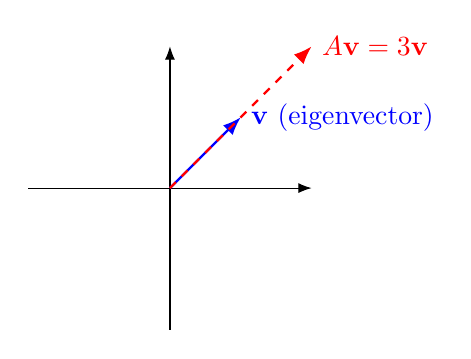
\begin{tikzpicture}[scale=0.9]
\draw[-{Latex}] (-2,0) -- (2,0);
\draw[-{Latex}] (0,-2) -- (0,2);
\draw[-{Latex}, thick, blue] (0,0) -- (1,1) node[right]{$\vect{v}$ (eigenvector)};
\draw[-{Latex}, thick, red, dashed] (0,0) -- (2,2) node[right]{$A\vect{v}=3\vect{v}$};
\end{tikzpicture}
\begin{block}{Interpretation}
\begin{itemize}
\item $A$ stretches $\vect{v}$ by a factor of $\lambda = 3$ but keeps it on the \textbf{same line} through the origin.
\item Non-eigenvectors, in general, get \textbf{rotated} as well as scaled by $A$.
\item Eigenvalues/eigenvectors are central to PCA, stability analysis, and many ML algorithms.
\end{itemize}
\end{block}
\end{frame}

% ================================================================
\section{Hyperplanes \& Weight Vectors}
% ================================================================

\begin{frame}{Hyperplanes and the Weight Vector}
\begin{block}{General Hyperplane Equation}
$$ax+by+c=0 \;(\text{line}), \qquad ax+by+cz+d=0\;(\text{plane})$$
$$\sum_{i=1}^{n} w_ix_i + \theta = 0 \quad \Longleftrightarrow \quad \vect{w}^T\vect{x}+\theta = 0$$
\end{block}
\begin{alertblock}{Key Fact}
$\vect{w}$ is called the \textbf{weight vector} of the hyperplane. For any hyperplane $\vect{w}^T\vect{x}=0$, the weight vector $\vect{w}$ is \textbf{always perpendicular} to the hyperplane.
\end{alertblock}
\begin{itemize}
\item Changing the weight vector $\vect{w}$ changes the \textbf{orientation} of the hyperplane.
\end{itemize}
\end{frame}

\begin{frame}{Hyperplane Diagram}
\centering
\begin{tikzpicture}[scale=1.0]
\draw[-{Latex}] (-2,0) -- (2,0);
\draw[-{Latex}] (0,-2) -- (0,2);
\draw[thick, blue] (-1.6,-1.6) -- (1.6,1.6) node[above right]{hyperplane: $w^Tx=0$};
\draw[-{Latex}, thick, red] (0,0) -- (-1,1) node[above left]{$\vect{w}$};
\draw (0.3,0) arc (0:135:0.3);
\end{tikzpicture}
\begin{block}{Interpretation}
\begin{itemize}
\item If, for a data point $\vect{x}$: $\vect{w}^T\vect{x} > 0$, it lies on one side; $\vect{w}^T\vect{x} < 0$, the other side.
\item This idea underlies linear classifiers (e.g. the Perceptron).
\end{itemize}
\end{block}
\end{frame}

% ================================================================
\section{Metric Space \& Inner Product Space}
% ================================================================

\begin{frame}{Metric Space}
\begin{block}{Definition}
A \textbf{metric space} is a set together with a \textbf{distance function} $d(\vect{x},\vect{y})$ that defines the distance between any two objects (points) in the set.
\end{block}
\begin{itemize}
\item Must satisfy: non-negativity, symmetry, and the triangle inequality.
\item Example distance: Euclidean distance $d(\vect{x},\vect{y}) = \|\vect{x}-\vect{y}\|$.
\end{itemize}
\end{frame}

\begin{frame}{Inner Product Space}
\begin{block}{Definition}
An \textbf{inner product space} is a vector space $V$ equipped with an inner product $\langle \vect{u},\vect{v}\rangle$ that aligns two mathematical objects with each other.
\end{block}
\begin{block}{Inner Product in $\R^n$}
$$\langle \vect{u},\vect{v}\rangle = u_1v_1+u_2v_2+\cdots+u_nv_n = \sum_{i=1}^n u_iv_i$$
\end{block}
\begin{itemize}
\item \textbf{Norm} of a vector: $\|\vect{v}\| = \sqrt{\langle \vect{v},\vect{v}\rangle}$ — the inner product of a vector with itself.
\item Inner product of \textbf{zero vectors} is $0$, and they are considered \textbf{orthogonal} ($\perp$): $\langle\vect{u},\vect{v}\rangle = 0 \Rightarrow$ orthogonal.
\end{itemize}
\end{frame}

\begin{frame}{Angle Between Vectors \& Cosine Similarity}
\begin{block}{Formula}
$$\cos\theta = \frac{\langle \vect{u},\vect{v}\rangle}{\|\vect{u}\|\,\|\vect{v}\|} \qquad \Longrightarrow \qquad \theta = \cos^{-1}\!\left[\frac{\langle \vect{u},\vect{v}\rangle}{\|\vect{u}\|\,\|\vect{v}\|}\right]$$
\end{block}
\begin{alertblock}{Cosine Distance / Similarity}
\begin{itemize}
\item Two vectors highly \textbf{similar}: $\cos\theta \to 1$ (pointing in nearly the same direction).
\item Two vectors highly \textbf{dissimilar}: $\cos\theta \to 0$ (near orthogonal).
\end{itemize}
\end{alertblock}
\begin{itemize}
\item Widely used in data science/ML (e.g. text and embedding similarity) to compare vectors regardless of magnitude.
\end{itemize}
\end{frame}

% ================================================================
\section{Perceptron: An Application}
% ================================================================

\begin{frame}{Perceptron — The Simplest Neural Network Model}
\centering
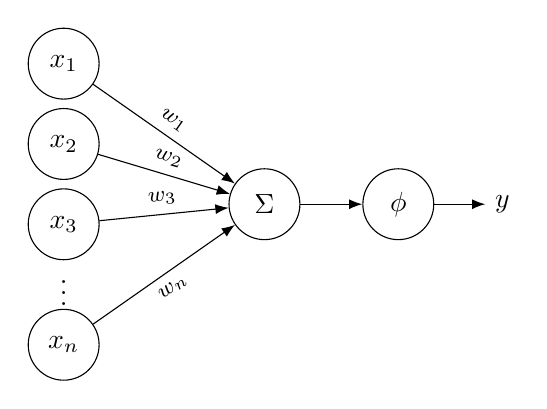
\begin{tikzpicture}[scale=0.85,
  neuron/.style={circle, draw, minimum size=0.9cm},
  sum/.style={circle, draw, minimum size=0.9cm}
]
\node[neuron] (x1) at (0,3) {$x_1$};
\node[neuron] (x2) at (0,1.8) {$x_2$};
\node[neuron] (x3) at (0,0.6) {$x_3$};
\node at (0,-0.3) {$\vdots$};
\node[neuron] (xn) at (0,-1.2) {$x_n$};

\node[sum] (sum) at (3,0.9) {$\Sigma$};
\node[neuron] (phi) at (5,0.9) {$\phi$};

\draw[-{Latex}] (x1) -- node[above, sloped]{\footnotesize $w_1$} (sum);
\draw[-{Latex}] (x2) -- node[above, sloped]{\footnotesize $w_2$} (sum);
\draw[-{Latex}] (x3) -- node[above, sloped]{\footnotesize $w_3$} (sum);
\draw[-{Latex}] (xn) -- node[below, sloped]{\footnotesize $w_n$} (sum);
\draw[-{Latex}] (sum) -- (phi);
\draw[-{Latex}] (phi) -- ++(1.3,0) node[right]{$y$};
\end{tikzpicture}
\end{frame}

\begin{frame}{Perceptron — Equations}
\begin{block}{Weighted Sum and Activation}
$$y = \phi\left(\sum_{i=1}^n w_ix_i - \theta\right) = \phi(\vect{w}^T\vect{x})$$
\end{block}
\begin{itemize}
\item $\vect{w}^T\vect{x}$ is exactly the \textbf{hyperplane} expression seen earlier — the perceptron classifies points based on which side of a hyperplane they fall on.
\item $\phi$ is the \textbf{activation function} (e.g. step function outputting $0$ or $1$).
\end{itemize}
\begin{block}{Output (binary classification)}
$$y(\vect{x}) = \begin{cases} 0 \\ 1 \end{cases}$$
\end{block}
\begin{itemize}
\item This directly connects \textbf{linear algebra} (dot products, hyperplanes, weight vectors) to \textbf{machine learning} models.
\end{itemize}
\end{frame}

% ================================================================
\section{Outliers (Quick Reference)}
% ================================================================

\begin{frame}{Outliers and IQR }
\begin{block}{Interquartile Range}
$$IQR = Q_3 - Q_1$$
\end{block}
\begin{alertblock}{Outlier}
Data which \textbf{stands away} from the rest of the group.
\end{alertblock}
\begin{block}{Outlier Rule (using IQR)}
A data point $x$ is an outlier if:
$$x < Q_1 - 1.5\,IQR \qquad \text{or} \qquad x > Q_3 + 1.5\,IQR$$
\end{block}
\begin{itemize}
\item Related shape measures: \textbf{Skewness} (asymmetry of the distribution) and \textbf{Kurtosis} (peakedness / tail-heaviness).
\end{itemize}
\end{frame}

\begin{frame}
\centering
\Huge Thank You!
\end{frame}

\end{document}